\documentclass[11pt,a4paper]{article}

\usepackage[margin=1in]{geometry}
\usepackage[T1]{fontenc}
\usepackage{lmodern}
\usepackage{microtype}
\usepackage{enumitem}
\usepackage{booktabs}
\usepackage{graphicx}
\usepackage[font=small,labelfont=bf]{caption}
\usepackage[colorlinks=true,linkcolor=blue,urlcolor=blue,citecolor=blue]{hyperref}
\usepackage{xurl}
\usepackage{titlesec}

\titleformat{\section}{\large\bfseries}{\thesection.}{0.6em}{}
\titleformat{\paragraph}[runin]{\normalfont\itshape}{}{0em}{}
\titlespacing*{\paragraph}{0pt}{6pt}{0.6em}
\setlist{itemsep=2pt,parsep=0pt,topsep=4pt}
\graphicspath{{figures/}}

% clickable in-text citation: \rc{5} -> jumps to reference [5]
\newcommand{\rc}[1]{\hyperlink{ref#1}{#1}}

\title{Progress Report\\[0.3em]
\large Data Preprocessing Pipeline and Model Direction}
\author{Ahmed Khader}
\date{22 July 2026}

\begin{document}

\maketitle

\begin{abstract}
\noindent This report covers two strands of work on the MIT-BIH arrhythmia data.
The first is the data preprocessing pipeline: I reviewed how the literature (six-plus
papers) prepares ECG signals, settled on a pipeline of wavelet denoising, per-patient
normalization, inter-patient splitting, and fixed window segmentation, and recorded why I
preferred a learned dimensionality reduction over PCA and ICA. The second strand is the model
direction for the forecasting task, where the chaotic nature of the problem in general, not
just the model, limits how far ahead we can predict, and where I argue for rethinking both the
model family and the evaluation criterion. Screenshots of the processing applied to the actual
data are included as Figures~\ref{fig:wavelet} and~\ref{fig:zscore}.
\end{abstract}

% =====================================================================
\section{Literature Review of Preprocessing}

I began the data analysis by surveying what the literature already does, gathering six-plus
papers whose links are listed in the References. Across them the preprocessing backbone is
remarkably consistent. Most pipelines start by removing noise (either with a notch filter,
with a combination of high- and low-pass filters, or with a wavelet-based denoiser), then
apply normalization, and finally perform window (segment) splitting. A subset of papers add a
dimensionality-reduction step, usually Principal Component Analysis (PCA). This common
structure, confirmed across both the survey papers~[\rc{5},\rc{6},\rc{7}] and the applied
forecasting and classification work~[\rc{1},\rc{2},\rc{3},\rc{4}], is what I used as the
template for my own pipeline.

% =====================================================================
\section{Dimensionality Reduction: Why I Preferred a Learned Approach}

\textit{PCA.} PCA reduces dimensionality by keeping the directions of greatest variance, which
means it describes the data purely through its covariance: a second-order, ellipsoidal
``shape.'' That description is complete only for a Gaussian distribution, whose shape is
exactly that ellipsoid. ECG is strongly non-Gaussian, with much of its information carried by
sparse, high-amplitude deflections (the QRS complex) that are higher-order structure the
covariance cannot see. PCA does not strictly require Gaussian data to run, but its notion of
``shape'' is the Gaussian one, so for a signal this non-Gaussian the leading components are not
guaranteed to be the most informative directions. That is why I preferred a learned
representation (Section~\ref{sec:tcn}) over a linear PCA projection, rather than a claim that
PCA cannot work on ECG at all.

\textit{ICA.} Independent Component Analysis is also common and is effective at isolating and
removing noise, but I chose not to build on it either. Its practical limits fit our setting
poorly: with only two leads, ICA can recover at most two components, which is weak for
separating more than two overlapping sources; its components carry arbitrary sign, scale, and
ordering; and it assumes the sources mix linearly, instantaneously, and stationarily. More
fundamentally, the independence assumption sits awkwardly on multi-lead ECG, because the leads
are largely different projections of the same cardiac dipole and are therefore highly
dependent, so the recovered ``independent'' components need not correspond to meaningful
physiological sources. Deciding which components are noise is also subjective, and discarding a
component that is not purely noise can remove genuine signal, not only
artifacts~[\rc{8}].

% =====================================================================
\section{The Adopted Preprocessing Pipeline}

In chronological order, my pipeline is: wavelet denoising, then normalization per patient,
then inter-patient splitting, then fixed window segmentation.

\paragraph{Wavelet denoising.} The wavelet transform is, in effect, mathematical magic for
this problem: a full treatment of the underlying equations is beyond the scope of this report,
but the intuition is simple. The transform decomposes the signal across scales. The coherent,
high-energy structure of the heartbeat concentrates into a few large coefficients, whereas
random noise, being random, spreads thinly across many small coefficients at many frequencies.
Thresholding away the small coefficients therefore strips out the noise while keeping the most
powerful part of the signal, the true waveform. Figure~\ref{fig:wavelet} shows this on real
data, including the removal of baseline wander.

\begin{figure}[ht]
  \centering
  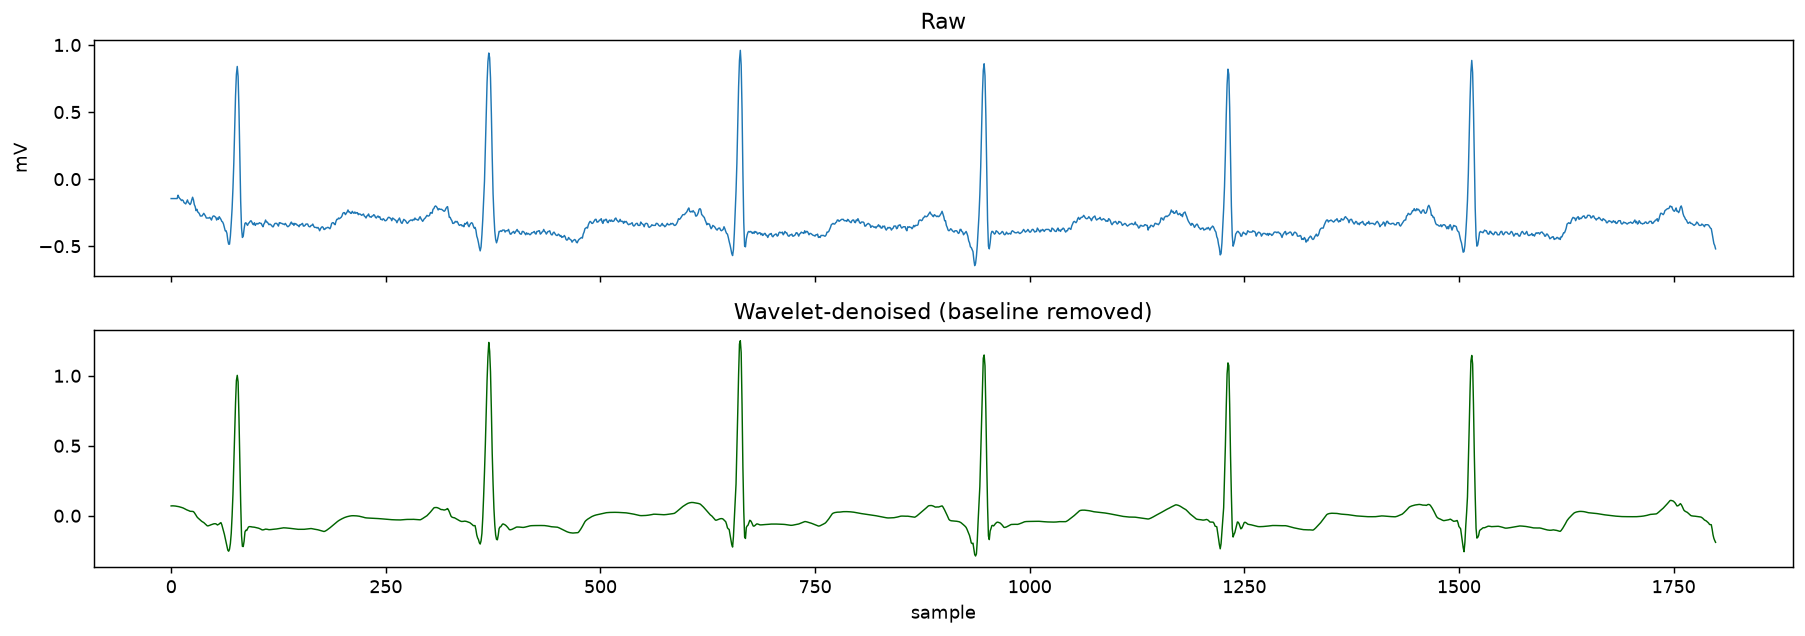
\includegraphics[width=\linewidth]{fig1_wavelet.png}
  \caption{Screenshot of the wavelet denoising applied to the data (record~100, first
  five seconds): raw signal (top) versus the wavelet-denoised signal with baseline
  wander removed (bottom).}
  \label{fig:wavelet}
\end{figure}

\paragraph{Normalization (per patient).} Normalization is then carried out on every patient
alone rather than across the whole dataset. This gives each record a consistent scale (zero
mean, unit variance) and, because the statistics never cross between patients, it cannot leak
information from one record into another. Figure~\ref{fig:zscore} shows the effect.

\begin{figure}[ht]
  \centering
  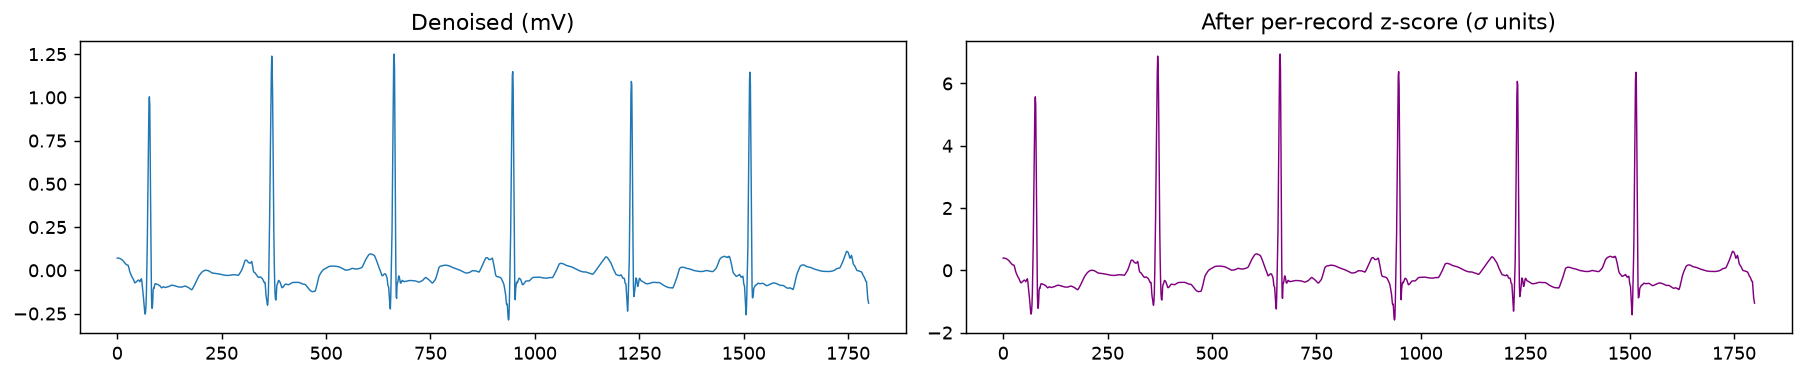
\includegraphics[width=\linewidth]{fig2_zscore.png}
  \caption{Screenshot of the normalization step (record~100): the denoised signal in
  millivolts (left) and the same signal after per-patient z-score normalization, now in
  standard-deviation units (right).}
  \label{fig:zscore}
\end{figure}

\paragraph{Inter-patient splitting.} The normalized records are then split at the patient
level (discussed in Section~\ref{sec:interpatient}).

\paragraph{Window segmentation.} Finally, the data is divided by fixed window splitting. Here
I followed the literature to the bone, using the standard fixed-size segmentation with an
$80/10/10$ train/validation/test division.

% =====================================================================
\section{Intra- versus Inter-Patient Evaluation}
\label{sec:interpatient}

I believe inter-patient evaluation is both the better and the more honest choice, and a review
paper in my references makes the same point~[\rc{7}]. The distinction is about how the data is
split. In the intra-patient setting the beats themselves are pooled and split, so a given
patient's beats can land in both the training and the test set. The model may then have
effectively already seen that patient's pattern during training and simply replicates it at
test time, which leaks information and inflates the result. Inter-patient evaluation instead
holds out whole patients for testing and trains and validates on different ones. That is the
true scenario we care about: a new patient arrives on their own, and we test the model on
them.

% =====================================================================
\section{TCN Encoder--Decoder for Dimensionality Reduction}
\label{sec:tcn}

Because PCA and ICA each fit this signal poorly for the reasons above, I adopted a
\emph{learned} dimensionality-reduction step instead: a temporal convolutional network (TCN)
autoencoder. Its encoder compresses each window (for example from $3600$ samples down to
roughly $600$) into a compact representation, so the downstream model trains faster, and it
learns that representation from the data rather than assuming a fixed statistical shape or an
independence structure. This follows an established line of work that uses convolutional and
TCN autoencoders to compress ECG into low-dimensional features for a downstream
model; my contribution is the specific configuration and, in particular, how far the
compression can be pushed before too much information is lost, which is still under
investigation.

% =====================================================================
\section{Future Work: Data Processing}

Remaining directions on the preprocessing side are to explore downsampling, to experiment with
the window size to find the right value (or else keep the literature's default), and to explore
the TCN encoder further.

% =====================================================================
\section{Model Direction and Open Thoughts}

Choosing the model is the hard part, and the deeper difficulty is not specific to ECG but to
chaotic systems in general, with ECG being one of the simplest cases. Our problem is
forecasting: we must predict the signal's values and, ideally, extend the horizon over which
those predictions stay accurate. In a chaotic system a tiny difference between the prediction
and the truth grows exponentially, at a rate set by the largest Lyapunov exponent, and throws
the two onto separate trajectories. That small difference is unavoidable, because both our
measurements and the model itself are approximations. The standard predictability scaling makes
the consequence precise: the usable horizon grows only like the \emph{logarithm} of the
accuracy, so even a model a thousand times more accurate buys only a little more
horizon.\footnote{The relevant scaling is $T \sim (1/\lambda)\ln(1/\delta)$ for initial error
$\delta$ and largest Lyapunov exponent $\lambda$; I am happy to share the derivation. My own
estimate of $\lambda$ on the MIT-BIH records was modest but positive across every record,
consistent with ECG being a comparatively mild case.}

The problem therefore lies partly in the model and partly in the nature of chaotic data, which
we cannot change. That leaves two options. Either we find a model that essentially cannot
mistake, or, more realistically, we change the evaluation itself. Instead of demanding that
every predicted number be exact, we can evaluate whether the prediction follows a
\emph{similar trajectory that settles onto the same attractor}: the overall behaviour is right
even if the individual numbers differ. In clinical terms, we would judge whether the model
correctly predicts, say, that a patient's heart is accelerating in the same way, not claiming
the patient is healthy, but capturing the dynamics.

With that framing, I am proposing to borrow from fields that already forecast chaotic,
high-dimensional systems. Weather forecasting is the closest analogue, and there the leading
systems use distinct architectures: 3D transformers (for example Pangu-Weather) and graph
neural networks (for example GraphCast), among others. My proposal is to investigate whether
these, alongside reservoir computing (which has a strong track record on chaotic systems such
as the Lorenz attractor), can be adapted to our problem:
\begin{itemize}
  \item Reservoir computing: reading the primary papers to understand its limitations more
        precisely.
  \item 3D transformers and graph neural networks from weather forecasting, treated as
        candidates to adapt rather than established solutions for ECG.
\end{itemize}
The next step is to study these approaches in depth and to look for a novel way of my own to
approach the problem.

% =====================================================================
\section*{References}
\addcontentsline{toc}{section}{References}
\begin{enumerate}[label={[\arabic*]},leftmargin=2.2em]
  \item \hypertarget{ref1}{}H.~Zacarias et al., ``ECG Forecasting System Based on Long
        Short-Term Memory,'' \emph{Bioengineering}, 2024.
        \url{https://www.mdpi.com/2306-5354/11/1/89}
  \item \hypertarget{ref2}{}Wang et al., ``Hybrid CNN-LSTM model for ECG-based arrhythmia
        detection in the internet of medical things,'' \emph{Discover Internet of Things},
        2025. \url{https://link.springer.com/article/10.1007/s43926-025-00131-7}
  \item \hypertarget{ref3}{}M.~Ruiz-Barroso et al., ``FADE: Forecasting for Anomaly Detection
        on ECG,'' \emph{Computer Methods and Programs in Biomedicine}, 2025.
        \url{https://www.sciencedirect.com/science/article/pii/S016926072500197X}
  \item \hypertarget{ref4}{}M.~Cao et al., ``ECG Heartbeat Classification using Deep Transfer
        Learning with Convolutional Neural Network and STFT Technique,'' arXiv:2206.14200,
        2022. \url{https://arxiv.org/abs/2206.14200}
  \item \hypertarget{ref5}{}T.~Ansari et al., ``Deep Learning for ECG Arrhythmia Detection and
        Classification: an Overview of Progress in 2020--2023,'' \emph{Frontiers in
        Physiology}, 2023.
        \url{https://www.frontiersin.org/journals/physiology/articles/10.3389/fphys.2023.1246746/full}
  \item \hypertarget{ref6}{}N.~Ebrahimi et al., ``A Review on Deep Learning Methods for ECG
        Arrhythmia Classification,'' \emph{Expert Systems with Applications: X}, 2020.
        \url{https://www.sciencedirect.com/science/article/pii/S2590188520300123}
  \item \hypertarget{ref7}{}E.~J.~da~S.~Luz et al., ``ECG-based Heartbeat Classification for
        Arrhythmia Detection: A Survey,'' \emph{Computer Methods and Programs in Biomedicine},
        2016. \url{https://www.sciencedirect.com/science/article/pii/S0169260715003314}
  \item \hypertarget{ref8}{}I.~Atti et al., ``Measuring the Accuracy of ICA-based Artifact
        Removal from TMS-evoked Potentials,'' \emph{Brain Stimulation}, 2024.
        \url{https://www.sciencedirect.com/science/article/pii/S1935861X23019629}
\end{enumerate}

\end{document}
